\documentclass[a4paper]{article}
\usepackage[french]{babel}
\usepackage[utf8]{inputenc}
\usepackage[T1]{fontenc}
\usepackage{graphicx}   % pour les images
\usepackage{hyperref}   % pour les références
\usepackage{amssymb}    % pour les symboles de maths comme \mathbb{R}
\usepackage{mathtools}  % pour rajouter \text dans un environment math
\usepackage{subcaption} % pour les subfigures
\usepackage{todonotes} 
\usepackage{float}


\title{Rapport PSTALN}
\author{Cléa Han, Yanis Labeyrie et Adrien Zabban}
\date{janvier 2024}

\begin{document}

\maketitle

\section{Introduction}

Le but de ce projet consistait à entraîner un modèle de langage à prédire certains attributs des mots d'une
phrase. Une des tâches sur lesquelles nous nous sommes concentrées est appelée le balisage de séquence
prototypique. Cette tâche consiste à attribuer des étiquettes à chaque élément d'une séquence en fonction
de son prototype ou modèle. Par exemple, dans le domaine de la reconnaissance d'entités nommées,
on pourrait avoir une phrase en français comme :

"Jean travaille chez Microsoft à Paris."    

Dans cette phrase, la tâche de balisage de séquence consisterait à attribuer des étiquettes à chaque mot,
indiquant s'il s'agit d'un nom propre, d'une entreprise, d'une localité, etc. Un exemple de balisage de
séquence prototypique (POS-tagging) pour cette phrase pourrait être :

"Jean [name] travaille [verb] chez [pronoun] Microsoft [noun] à [pronoun] Paris [noun]."

Ici, chaque mot est étiqueté en fonction de son prototype ou de sa catégorie, ce qui permet de comprendre
le rôle de chaque élément dans la séquence. 

Nous nous sommes également concentrés sur une autre tâche: la prédiction des traits morpho syntaxiques.
Par exemple prédire à quel personne est un verbe, si un nom est au pluriel, ect..


\section{Dataset d'entraînement et préparation des données}

Parler ici du dataset, comment il est traité, le padding, les mots inconnus ....

\subsection{Gestion des OOV}

Pour gérer les OOV (les mots qui ne sont pas dans le vocabulaire d'entrainement, nous avons décidé de leur
attribuer un token particulié: le token <UNK>. L'ennui est qu'il faut attribuer un embedding à ce nouveau 
token, et qu'il faut également que cet embedding soit cohérent vis-à-vis des autres embeddings (on ne peut donc 
lui donner une valeur nulle ou aléatoire). L'idée est donc de construire cet embedding pendant l'entrainement en 
considérant qu'une proportion $f$ aléatoire des mots du dataset d'entrainement (nous avons pris f=1\%) sont des 
mots inconnus. Ceci permet au modèle d'apprendre un embedding cohérent pour le token <UNK> et donc de ne pas 
être "surpris" si il le rencontre en phase de test et de le gérer correctement.

\subsection{Padding}

Les phrases données au réseau LSTM doivent être toutes exactement de la même longueur pendant l'entraînement. 
Pour cela nous créons donc des tokens <PAD> pour équilibrer les longeurs des phrases. L'embedding associé à ce 
token est naturellement le vecteur nul car ce token ne contient pas d'information. 


\section{Méthodologie et Modèle}


\subsection{Architecture du modèle}
Pour réaliser cette tâche nous avons opté pour l'utilisation d'un réseau de neurone récurent de type LSTM 
(Long-Short Term Memory) bidirectionnel. En effet, cette approche classique est intéressante car le résau 
LSTM bidirectionnel permet d'analyser les dépendances entre les mots potentiellement éloignés d'une phrase, 
or ceci est nécessaire pour démêler les ambiguïtés lors de l'étiquetage morpho-syntaxie. Considérons l'exemple 
suivant :

Phrase : "Je ne peux pas ouvrir le fichier que tu m'as envoyé."

Sans la capacité de capturer les dépendances à long terme, une approche classique pourrait avoir du mal à 
démêler l'ambiguïté dans la phrase, en particulier en ce qui concerne le mot "que". Est-ce une conjonction 
de subordination introduisant une proposition subordonnée relative, ou est-ce une conjonction de coordination?

Avec un réseau LSTM bidirectionnel, on peut mieux gérer ces dépendances à long terme. Le réseau peut prendre 
en compte le contexte des mots précédents et suivants pour déterminer que "que" est utilisé comme une 
conjonction de subordination dans ce cas précis. L'utilisation de la bidirectionnalité permet au modèle 
d'avoir une compréhension contextuelle plus riche, en analysant à la fois les mots antérieurs et postérieurs 
pour chaque position dans la séquence. 

Le réseau LSTM que nous avons employé est constitué d'un module LSTM bidirectionnel (comprenant 2 couches avec 
2 directions opposées) ainsi que d'une couche dense de $[n_neurone]$ qui récupère l'état caché de la dernière 
cellule LSTM est produit le vecteur des prédictions. 

\subsubsection{Architecture pour le POS-tagging}
Nous utilisons la CrossentropyLoss pour comparer les vecteurs de densité de probabilité de classe prédit par 
le modèle (un pour chaque mot de la phrase avec le vecteur one-hot correspondant à la vrai classe du mot).
Nous prédisons un nombre $[n_classes]$ d'attributs de POS-tagging possibles. 

\subsubsection{Architecture pour la prédiction de traits morphologiques}
Pour la tâche de prédiction des traits morphologiques, la difficulté est supérieure. En effet pour cette tâche 
il faut pour chaque mot de la phrase prédire à la fois son rôle dans la phrase (Verbe, Nom, ect..) mais aussi 
pour chacune de ses classes prédire des attributs (singulier, pluriel, ...).

Pour cela une première méthode serait d'entraîner un modèle distinct par attributs, mais cela demanderai un 
assez long temps d'entraînement. Nous avons donc opté pour une première méthode différente: prédire non pas un 
vecteur comme pour la première tâche mais une matrice [classe,attribut] sans changer l'architecture du réseau, 
simplement en changeant le nombre de neurones de la couche dense. Nous avons par la suite tenté une deuxième 
approche: diviser la sortie de la couche dense en la faisant passer dans un nombre n de couche dense égal au 
nombre de classes, chacune chargée de prédire un attribut et reformer la matrice après passage dans ces couches 
distinctes. L'intéret de cette approche est que l'on utilise les features extraites du bloc LSTM de manière 
commune pour les sous-tâches mais chaque sous-tâche de classification est réalisé par une couche dense distincte.

La fonction de coût utilisé est toujours la CrossentropyLoss mais elle est appliquée cette fois-ci classe par 
classe puis ensuite moyennée pour obtenir la valeur de loss globale.

\subsubsection{Problèmes rencontrés / Subtilités techniques}



\section{Résultats et métriques}

\todo{Parler ici des différentes métriques macro/micro/accuracy}

\subsection{Résultats et métriques pour le POS-tagging}
Nous avons donc lancé un entraînement de notre réseau LSTM-Bidirectionel sur 30 epochs pour le POS-tagging et 
nous avons obtenu une accuracy de validation d'environ 90\% ce qui dénote que le réseau à réussi à apprendre 
correctement cette tâche d'étiquetage, comme le montre la figure suivante:

\begin{figure}[H]
    \centering
    \begin{subfigure}{0.45\textwidth}
        \centering
        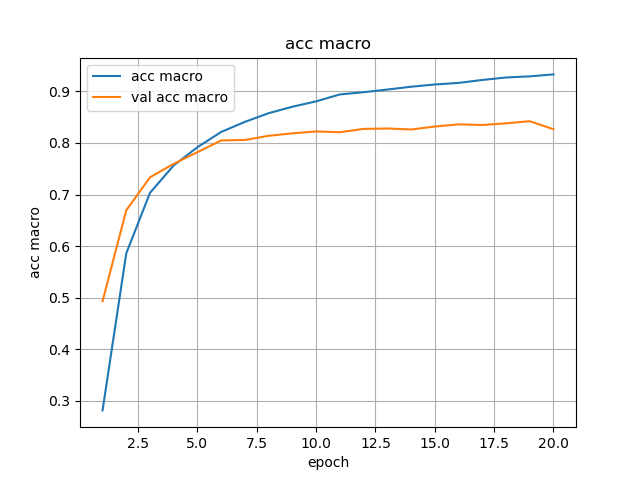
\includegraphics[width=\linewidth]{../logs/get_pos_French_2/acc macro.png}
        \caption{Valeurs de l'accuracy d'entraînement et de validation par epochs.}
    \end{subfigure}
    \hfill
    \begin{subfigure}{0.45\textwidth}
        \centering
        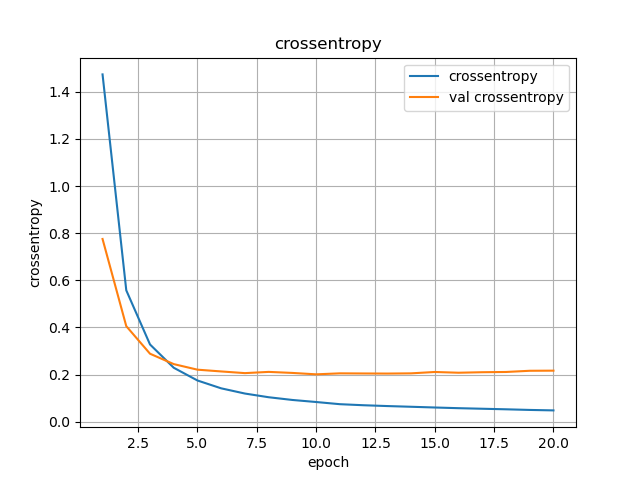
\includegraphics[width=\linewidth]{../logs/get_pos_French_2/crossentropy.png}
        \caption{Valeurs de la fonction de coût par epochs.}
    \end{subfigure}
    \caption{Comparaison des récompenses cumulées sur 100 étapes}
\end{figure}

On constate que la valeur de l'accuracy de validation est un peu plus faible que celle d'entraînement, cela 
s'explique par plusieurs facteurs, notamment la difficulté du modèle à généraliser aux nouveaux mots inconnus.

\subsection{Résultats et métriques pour la prédiction des traits morphologiques}

La tâche de prédiction des traits morphologiques comporte une subtilité: toutes les classes n'ont pas le même 
nombre d'attributs. Par exemple la classe "VERB" a 5 attributs tandis que la classe "NOUN" en a 12. Or, le 
réseau ne
peut pas prédire un vecteur de taille variable. Pour résoudre ce problème, nous avons donc décidé de rajouter 
des attributs fictifs à certaines classes pour que toutes les classes aient le même nombre d'attributs. Pour 
ce faire 
deux solutions sont possibles: soit chacune des sous-couches dense du réseau a le même nombre de neurones, et 
dans ce cas on rajoute des attributs fictifs et inutiles à certaines classe,
soit on définit des couches dense de tailles différentes pour chaque classe égales au noombre d'attributs de 
la classe, mais dans ce cas, il faut rajouter
du padding à la sortie de la couche dense pour que toutes les sorties aient la même taille. Nous avons testé 
les deux méthodes (qu'on appelera $"separate"$ pour la méthode sans padding et $"separate_0"$ pour la méthode 
avec padding après couche et nous avons obtenu de meilleurs résultats avec la deuxième méthode:

Pour la tâche de prédiction des traits morphologiques avec la méthode $separate_0$, nous obtenons les résultats 
suivants: %plot accuracy et crossentropy

\begin{figure}[H]
    \centering
    \begin{subfigure}{0.45\textwidth}
        \centering
        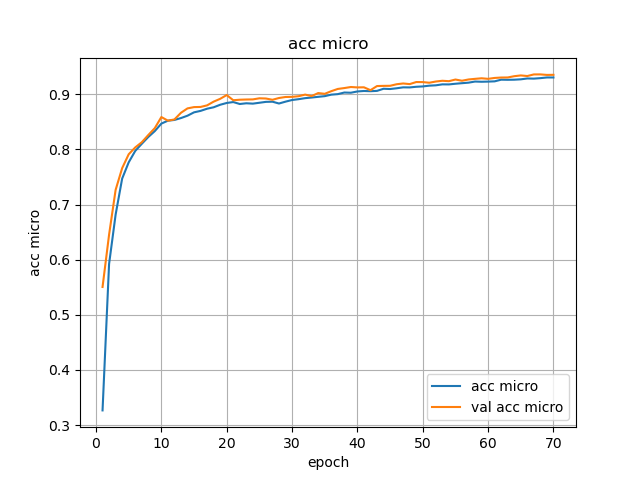
\includegraphics[width=\linewidth]{../logs/get_morphy_sep0_French_3/acc micro.png}
        \caption{Valeurs de l'accuracy d'entraînement et de validation par epochs.}
    \end{subfigure}
    \hfill
    \begin{subfigure}{0.45\textwidth}
        \centering
        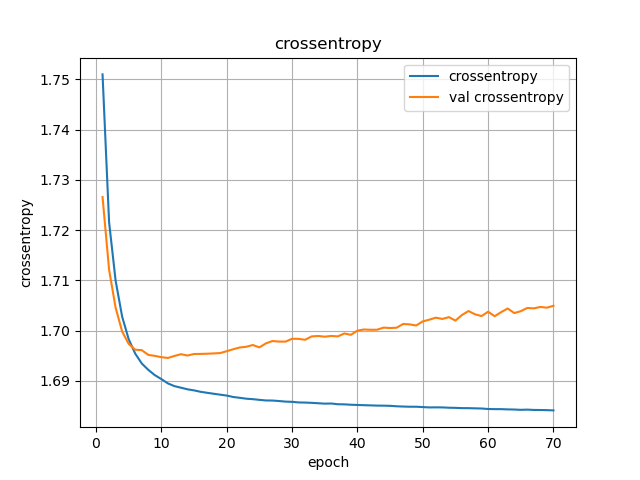
\includegraphics[width=\linewidth]{../logs/get_morphy_sep0_French_3/crossentropy.png}
        \caption{Valeurs de la fonction de coût par epochs.}
    \end{subfigure}
    \caption{Courbes d'accuracy et de crossentropy pour la tâche de prédiction des traits morphologiques}
\end{figure}

On mesure également une autre métrique appelée 'allgood' qui mesure le nombre de mots dont tous les attributs 
ont été prédits correctement. On obtient une valeur de allgood de: VALEUR comme le
montre la figure suivante:

\begin{figure}[H]
    \centering
    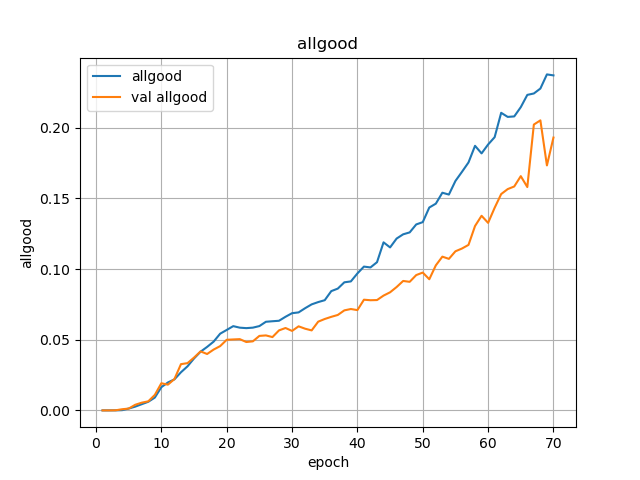
\includegraphics[width=0.45\linewidth]{../logs/get_morphy_sep0_French_3/allgood.png}
    \caption{Valeurs de la métrique allgood par epochs.}
\end{figure}


L'entraînement requiert un temps plus long que pour la tâche de POS-tagging car il y a beaucoups plus 
d'attributs à prédire.
On obtient une accuracy de validation final de VALEUR, et les courbes montrent que le modèle subit un 
léger sur-apprentissage (comme le montre la valeur de la loss de validation).

Pour la tâche de prédiction des traits morphologiques avec la méthode $separate$, nous obtenons les 
résultats suivants: %plot accuracy et crossentropy

\begin{figure}[H]
    \centering
    \begin{subfigure}{0.45\textwidth}
        \centering
        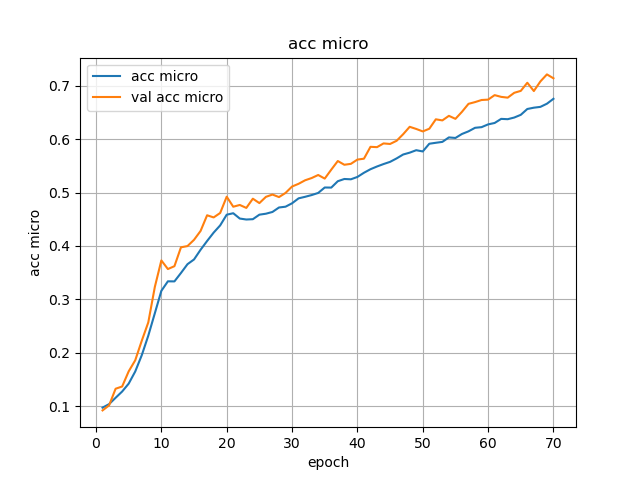
\includegraphics[width=\linewidth]{../logs/get_morphy_separate_French_1/acc_micro.png}
        \caption{Valeurs de l'accuracy d'entraînement et de validation par epochs.}
    \end{subfigure}
    \hfill
    \begin{subfigure}{0.45\textwidth}
        \centering
        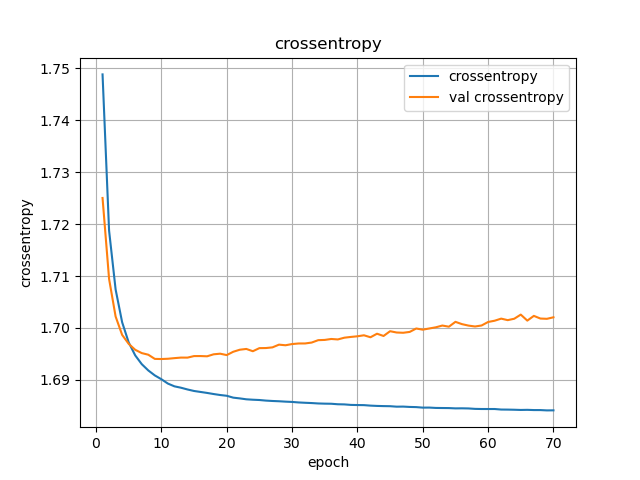
\includegraphics[width=\linewidth]{../logs/get_morphy_separate_French_1/crossentropy.png}
        \caption{Valeurs de la fonction de coût par epochs.}
    \end{subfigure}
    \caption{Courbes d'accuracy et de crossentropy pour la tâche de prédiction des traits morphologiques}
\end{figure}

On constate que les résultats sont moins bons que pour la méthode $separate_0$ et que le modèle a besoin de 
plus d'epochs. Cela s'explique par le fait que les attributs fictifs rajoutés aux classes 
pour que toutes les classes aient le même nombre d'attributs sont des attributs inutiles qui n'apportent pas 
d'information au modèle et qui peuvent donc le perturber.














\todo{Mettre ici le graphe d'entrainement}
\todo{Mettre ici des exemples d'inférences (un cas simple, un cas difficile ambigu}

En revanche pour la tâche de prédiction des traits morphologiques les résultats se sont avérés bien inférieurs avec une accuracy de validation de seulement 20%




\end{document}
